% -*- mode:latex; mode:flyspell -*-
\documentclass{beamer}[10pt]

% Copyright 2004 by Till Tantau <tantau@users.sourceforge.net>.
%
% In principle, this file can be redistributed and/or modified under
% the terms of the GNU Public License, version 2.
%
% However, this file is supposed to be a template to be modified
% for your own needs. For this reason, if you use this file as a
% template and not specifically distribute it as part of a another
% package/program, I grant the extra permission to freely copy and
% modify this file as you see fit and even to delete this copyright
% notice. 

\mode<presentation> {
  % \usetheme{Warsaw}
  \usetheme{Madrid}
%  \usetheme{Darmstadt}
%  \usetheme{Berkeley}
  % or ...

%  \setbeamercovered{transparent}
  % or whatever (possibly just delete it)
}

\usepackage[english]{babel}
% or whatever

\usepackage[latin1]{inputenc}
% or whatever

\usepackage{hyperref}
\usepackage{cancel}
\usepackage{tikz}
\usetikzlibrary{arrows}
\usetikzlibrary{decorations.markings}
\usetikzlibrary{decorations.pathmorphing}
% \usepackage[absolute,overlay]{textpos}
% \usepackage{onimage}
\usepackage{times}
\usepackage{graphics}
% \usepackage{subfigure}
% \usepackage{scalefnt}
%\usepackage{hyperref}
% \renewcommand\thesubfigure{\arabic{subfigure}}

\graphicspath{{figures}}

% \usepackage{pgfpages}
% \pgfpagesuselayout{2 on 1}[letterpaper,border shrink=2mm,landscape]

% make beamer and subfigure work well
\makeatletter
\def\ext\@subfigure{lof}
\makeatother

% \usepackage{geometry}
% \geometry{letterpaper,landscape}

% \usepackage{caption}
\usepackage[T1]{fontenc}
\usepackage{mathtools}

\usepackage{eso-pic}
%%%%%%%%%%%%%%%%%%%%%%%%%%%%%%%%%%%%%%%%%%%%%%%%%%%%%%%%%%%%%%%%%%%%%%%%%%%%%%%
\usecolortheme{rose}
\definecolor{coolblack}{rgb}{0.0, 0.18, 0.39}
\definecolor{UBCblue}{rgb}{0.0, 0.18, 0.39} % UBC Blue (primary)
\definecolor{UBCgrey}{rgb}{0.3686, 0.5255, 0.6235} % UBC Grey (secondary)
\setbeamercolor{palette primary}{bg=UBCblue,fg=white}
\setbeamercolor{palette secondary}{bg=UBCblue,fg=white}
\setbeamercolor{palette tertiary}{bg=UBCblue,fg=white}
\setbeamercolor{palette quaternary}{bg=UBCblue,fg=white}
\setbeamercolor{structure}{fg=UBCblue} % itemize, enumerate, etc
\setbeamercolor{section in toc}{fg=UBCblue} 
\setbeamertemplate{headline}{}
\setbeamertemplate{itemize items}[circle]
\setbeamertemplate{enumerate items}[default]
%\setbeamertemplate{footline}[frame number]
\setbeamertemplate{frametitle}[default][center]
\usefonttheme{serif}
%%%%%%%%%%%%%%%%%%%%%%%%%%%%%%%%%%%%%%%%%%%%%%%%%%%%%%%%%%%%%%%%%%%%%%%%%%%%%%%
% Or whatever. Note that the encoding and the font should match. If T1
% does not look nice, try deleting the line with the fontenc.

\title[TDAQ \& VST]{
  {
%  \vspace{-1.0 in}
    \bf {Collaboration Meeting: TDAQ Update} }
}




% \institute{\inst{1}Univ of Athens, \inst{2}Fermilab , \inst{3}Univ of Glasgow}

\author[Sara Gamba]{
  \fontseries{s}
  \selectfont
  { Sara Gamba, University of Pisa \\ \vspace{4mm} Presenting on behalf of Tracker DAQ group: \\ P. Murat (FNAL), M. Tecchio (University of Michigan), R. Bonventre (LBNL), V. Rusu (FNAL)}
}

% \date{\today}
\date{March 18th 2024}
% - Use the \inst command only if there are several affiliations.
% - Keep it simple, no one is interested in your street address.

% - Either use conference name or its abbreviation.
% - Not really informative to the audience, more for people (including
%   yourself) who are reading the slides online


% This is only inserted into the PDF information catalog. Can be left
% out. 

% If you have a file called "university-logo-filename.xxx", where xxx
% is a graphic format that can be processed by latex or pdflatex,
% resp., then you can add a logo as follows:

%%% \pgfdeclareimage[height=0.5cm]{university-logo}{checks\_reorder.pdf}
%%% \logo{\pgfuseimage{university-logo}}

% Delete this, if you do not want the table of contents to pop up at
% the beginning of each subsection:
%%\AtBeginSubsection[] {
%%%------------------------------------------------------------------------------
%% \begin{frame}<beamer>{\underline{Outline}}
%%    % \tableofcontents[currentsection,currentsubsection]
%%  \tableofcontents[currentsection]
%% \end{frame}
%%}
%%

% If you wish to uncover everything in a step-wise fashion, uncomment
% the following command: 

% \beamerdefaultoverlayspecification{<+->}

\hypersetup{%
  colorlinks=UBCblue,% hyperlinks will be black
  linkbordercolor=UBCblue,% hyperlink borders will be red
  pdfborderstyle={/S/U/W 1}% border style will be underline of width 1pt
}

%%%%%%%%%%%%%%%%%%%%%%%%%%%%%%%%%%%%%%%%%%%%%%%%%%%%%%%%%%%%%%%%%%%%%%%%%%%%%%%
% COMMANDS
%%%%%%%%%%%%%%%%%%%%%%%%%%%%%%%%%%%%%%%%%%%%%%%%%%%%%%%%%%%%%%%%%%%%%%%%%%%%%%%
\newcommand {\baftwo}        {\mbox{$BaF_2$}}
\newcommand {\blue}          {\color{blue}}
\newcommand {\deltaE}        {\mbox{$\delta{\rm-electron}$}}
\newcommand {\eemm}          {\mbox{$ee\mu\mu$}}
\newcommand {\et}            {\mbox{$E_T$}}
\newcommand {\etcorr}        {\mbox{$E_T^{corr}$}}
\newcommand {\gevcsq}        {\mbox{$GeV\!/c^2$}}
\newcommand {\gt}            {\mbox{$>$}}
\newcommand {\invfb}         {\mbox{$fb^{-1}$}}
\newcommand {\invfbrm}       {\mbox{$\rm fb^{-1}$}}
\newcommand {\invpb}         {\mbox{$pb^{-1}$}}
\newcommand {\invpbrm}       {\mbox{$\rm pb^{-1}$}}
\newcommand {\jpsi}          {\mbox{$J/\psi$}}
\newcommand {\lt}            {\mbox{$<$}}
\newcommand {\met}           {\mbox{${\not\! E}_{T}$}}
\newcommand {\mmmm}          {\mbox{$\mu\mu\mu\mu$}}
\newcommand {\mzz}           {\mbox{$M_{ZZ}$}}
\newcommand {\pb}            {\mbox{\rm\,pb}}
\newcommand {\ppbar}         {\mbox{$p\bar{p}$}}
\newcommand {\pt}            {\mbox{$p_T$}}
\newcommand {\red}           {\color{red}}
\newcommand {\stat}          {\mbox{\rm (stat.)}}
\newcommand {\statsys}       {\mbox{\rm (stat.+syst.)}}
\newcommand {\syst}          {\mbox{\rm (syst.)}}
\newcommand {\wpigamma}      {\mbox{$W^{\pm} \rightarrow \pi^{\pm} \gamma$}}
\newcommand {\wenu}          {\mbox{$W^{\pm} \rightarrow e^{\pm} \nu$}}
\newcommand {\wlnu}          {\mbox{$W^{\pm} \rightarrow l^{\pm} \nu$}}
\newcommand {\wmunu}         {\mbox{$W^{\pm} \rightarrow \mu^{\pm} \nu$}}
\newcommand {\wtaunu}        {\mbox{$W^{\pm} \rightarrow \tau^{\pm} \nu$}}
\newcommand {\zpsigamma}     {\mbox{$    Z^{0} \rightarrow J/\psi \gamma$}}
\newcommand {\zpigamma}      {\mbox{$\rm Z^{0} \rightarrow \pi^{0} \gamma$}}
\newcommand {\zee}           {\mbox{$\rm Z^0 \rightarrow e^+ e^-$}}
\newcommand {\zmumu}         {\mbox{$\rm Z^0 \rightarrow \mu^+ \mu^-$}}
\newcommand {\ztautau}       {\mbox{$\rm Z^0 \rightarrow \tau^+ \tau^-$}}
\newcommand {\zll }          {\mbox{$Z       \rightarrow l^{+}l^{-}$}}
\newcommand {\zupsgamma}     {\mbox{$    Z^0 \rightarrow \Upsilon \gamma$}}
\newcommand {\zzx }          {\mbox{$X       \to ZZ$}}
\newcommand {\zzllll}        {\mbox{$ZZ \to \ell^+ \ell^- \ell^+ \ell^-$}}
\newcommand {\zzllnn}        {\mbox{$ZZ \to \ell^+ \ell^- \nu \nu$}}
\newcommand {\zzlljj}        {\mbox{$ZZ \to \ell^+ \ell^- j j$}}

%\newcommand {\plots}  {/home/murat/figures}   % MURAT03

   % MURAT05
% \newcommand {\plots}  {/home/murat/figures/drs4}   % MURAT03


\begin{document}

%------------------------------------------------------------------------------
% working document - no title page
%------------------------------------------------------------------------------
% \begin{frame}
%   \titlepage
% \end{frame}
% -------------------------------------- uncomment this to get the table of contents 
% \begin{frame}{\underline{Outline}}
% \tableofcontents % [pausesections]
%  % You might wish to add the option [pausesections]
% \end{frame}
% 
%------------------------------------------------------------------------------
% \AtBeginSection[] {
%    \begin{frame}<beamer>{}
     %     \tableofcontents[currentsection,currentsubsection]
%    \tableofcontents[currentsection]
%    \end{frame}
% }
% 
% Structuring a talk is a difficult task and the following structure
% may not be suitable. Here are some rules that apply for this
% solution: 

% - Exactly two or three sections (other than the summary).
% - At *most* three subsections per section.
% - Talk about 30s to 2min per frame. So there should be between about
%   15 and 30 frames, all told.

% - A conference audience is likely to know very little of what you
%   are going to talk about. So *simplify*!
% - In a 20min talk, getting the main ideas across is hard
%   enough. Leave out details, even if it means being less precise than
%   you think necessary.
% - If you omit details that are vital to the proof/implementation,
%   just say so once. Everybody will be happy with that.
%%%%%%%%%%%%%%%%%%%%%%%%%%%%%%%%%%%%%%%%%%%%%%%%%%%%%%%%%%%%%%%%%%%%%%%%%%%%%%%

\begin{frame}
\centering
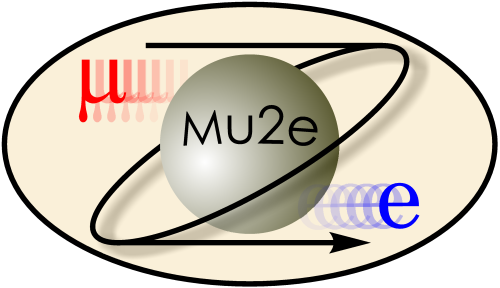
\includegraphics[height=1cm]{figures/png/mu2e_logo_oval.png}
\titlepage
\centering

\includegraphics[height=1cm]{figures/png/FNAL-Logo-NAL-Blue.png}\hspace{10mm}
\includegraphics[height=1.6cm]{figures/pdf/cherubino.pdf}

\end{frame}



ci sono istogrammi per errori
global run details: prima instabile 
abbiamo ancora il firmware vecchio su daq09
non ancora testato ilsoftware nuobo e accennare il rate ma non e un problema perche possiamo continuare a caratterizzare abbastanza bene l apparato (artdaq non e stato testato a quei rate) e pure slow control
daq is composed of controlling, monitoring and data flowing
gains, voltages devono essere controllati
slide con immagine del tracker board : hardware building that dtc-dtc connection
event building avverra nel dtc , not for cosmics
to be done: implementare lo slow control dei lowhigh voltage
\begin{frame}{A snapshot of the current job}
\vspace{-3mm}
\begin{itemize}
\item Currently in the phase of commissioning and integration;
\vspace{3mm}
\item Reading from a tracker station is imminent;
\vspace{3mm}
\item We need to know how to read the detector;
\vspace{3mm}
\item Learning about errors and data transmission;
\vspace{3mm}
\item A functional DAQ is needed.
\vspace{5mm}
\end{itemize}
$\Rightarrow$ The rest of the talk will be about \textbf{Data Quality Monitoring}
\\
\vspace{5mm}
$\Rightarrow$ Some updates form \textbf{GR1} will be given too
\end{frame}
\begin{frame}{Working area}
    \begin{columns}
        \begin{column}{0.5\framewidth}
            \begin{figure}[H]
                \centering
                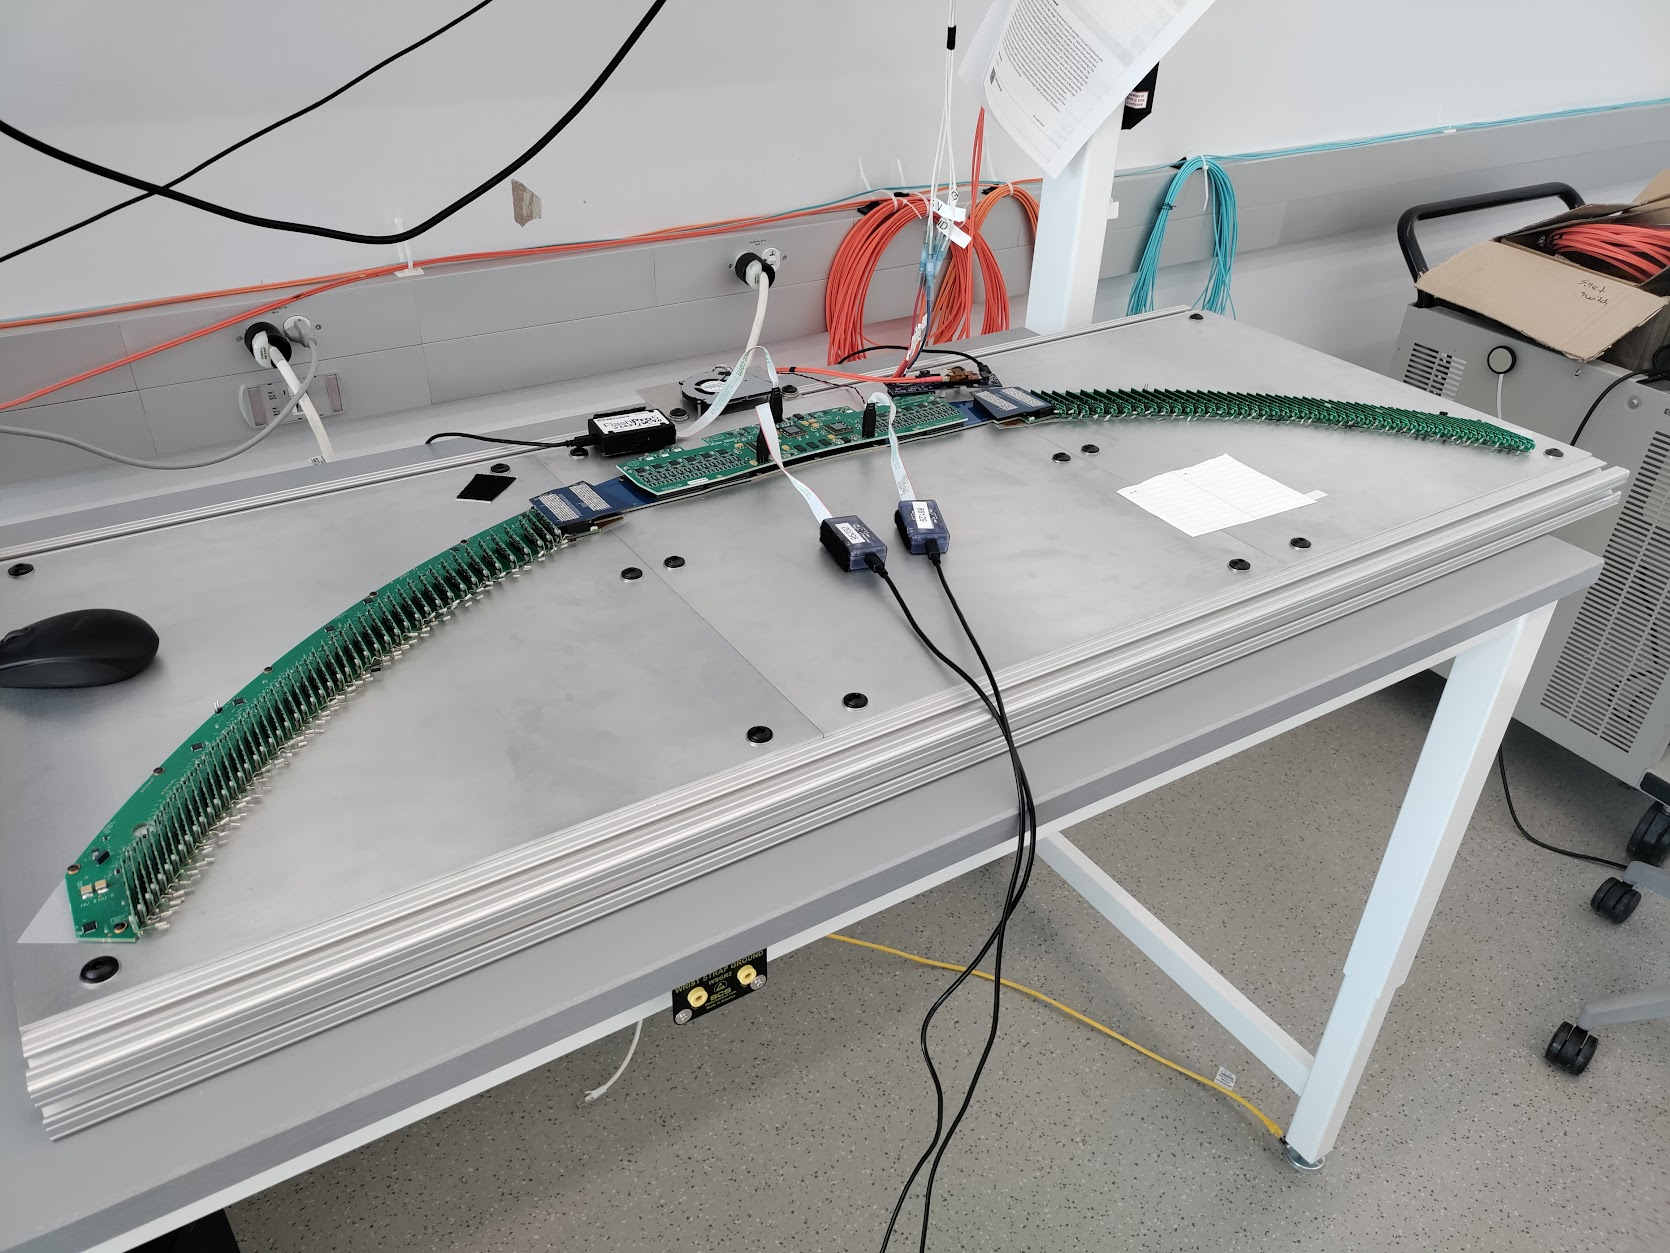
\includegraphics[width= \columnwidth]{figures/jpg/IMG_20240219_090538.jpg}
                \label{fig:enter-label}
            \end{figure}
\vspace{2mm}
            \begin{itemize}
            \item 3 test stands @IERC (only 2 have been used).
            \end{itemize}
        \end{column}
        \begin{column}{0.5\framewidth}
            \begin{itemize}
            \item DRAC card connected to the DTC installed in the DAQ computer mu2edaq09 via optical fibers;
\vspace{2mm}
            \item Each teststand has 96 channels;
\vspace{2mm}
            \item A pulser implemented in the DRACs is sending pulses to the preamps (CAL side) at 50 kHz;
\vspace{2mm}
            \item Pulses are digitized at 40 MHz;
\vspace{2mm}
            \item 12 channels pulsed per RUN;
\vspace{2mm}
            \item We are using 1 or 2 ROCs at the same time.
            \end{itemize}
        \end{column}
    \end{columns}
    \vspace{5mm}
\end{frame}

\begin{frame}{Description of the teststand setup}
 \begin{figure}[H]
   \centering
   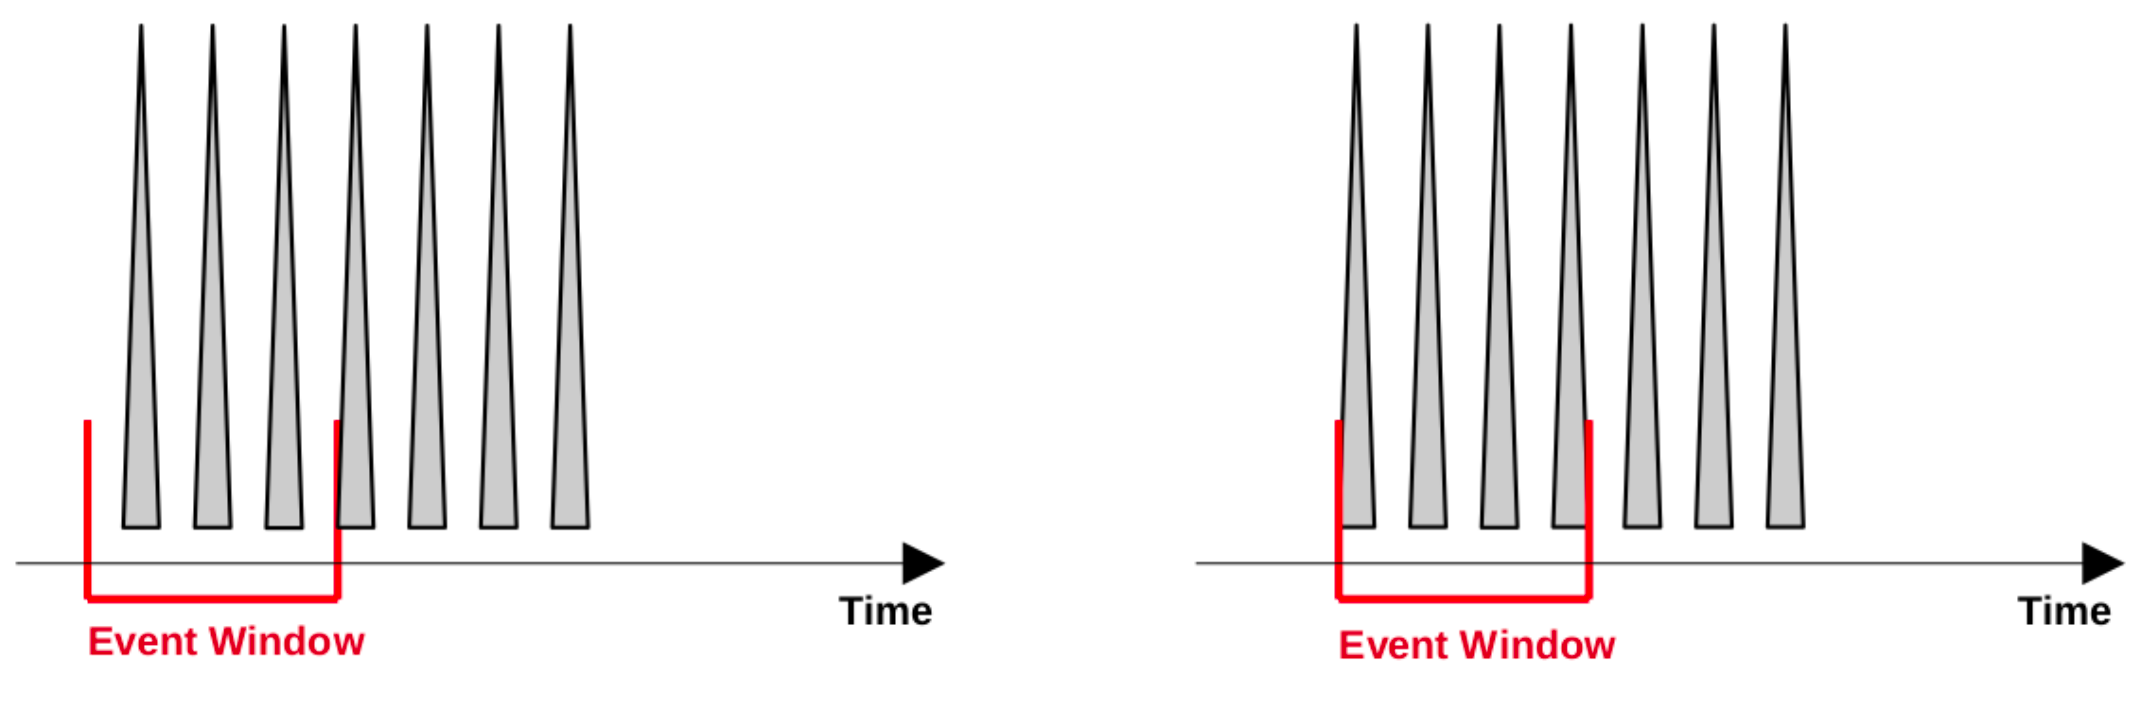
\includegraphics[width= 1.0\textwidth]{figures/png/Screenshot_20240308_165327.png}
   \label{fig:djn}
 \end{figure}
\begin{itemize}
\item Pulses are separated by 1/$f_{gen}$;
\item EW can be varied between 700 ns and 50 $\mu$s;
\item The timing of the readout is uncorrelated with the generator timing sequences$\rightarrow$number of readout pulses is variable;
\item ROC is reading digiFPGAs;
\item ROC hit buffer stores up to 255 hits (\href{https://mu2e-docdb.fnal.gov/cgi-bin/sso/RetrieveFile?docid=47837&filename=mu2e-47837.pdf&version=1}{DOCDB47837});
\item The channel readout sequence is fixed.
\end{itemize}
\end{frame}

\begin{frame}{Available Histograms and Error Identification}
\begin{columns}
\begin{column}{0.5\framewidth}
Real Time Monitoring:
\begin{itemize}
\item  \textbf{Channel histograms}:
\begin{itemize}
\item Time distribution of hits;
\item Waveforms;
\item First sample, baseline, charge, pulse height, charge tail and mean time distribution;
\item $\Delta t$ distribution between hits.
\end{itemize}
\item \textbf{ROC histograms}:
\begin{itemize}
\item Number of hits versus channel;
\item Waveform mean values versus channel. 
\end{itemize}
\item \textbf{Event histograms}:
\begin{itemize}
\item Number of hits distribution;
\item Error distribution;
\item Number of bytes distribution.
\end{itemize}
\end{itemize}
\end{column}
\begin{column}{0.5\framewidth}
Real Time Diagnostic:
\vspace{6mm}
\begin{itemize}
\item Number of bytes error bit; 
\vspace{4mm}
\item Number of ADC packets > 2;
\vspace{4mm}
\item Undefined link ID;
\vspace{4mm}
\item Invalid channel ID;
\vspace{4mm}
\item More hits than the maximum in a given channel.
\end{itemize}
\end{column}
\end{columns}
\end{frame}


\begin{frame}{Number of hits versus channel number}
\begin{columns}
\begin{column}{0.5\framewidth}
\vspace{-2mm}
\begin{itemize}
\item Need to see cross talks between channels:
\\
$\Rightarrow$ one pulsed channel for every eight not pulsed channels.
\end{itemize}
\vspace{-4mm}
\begin{figure}[H]
   \centering
   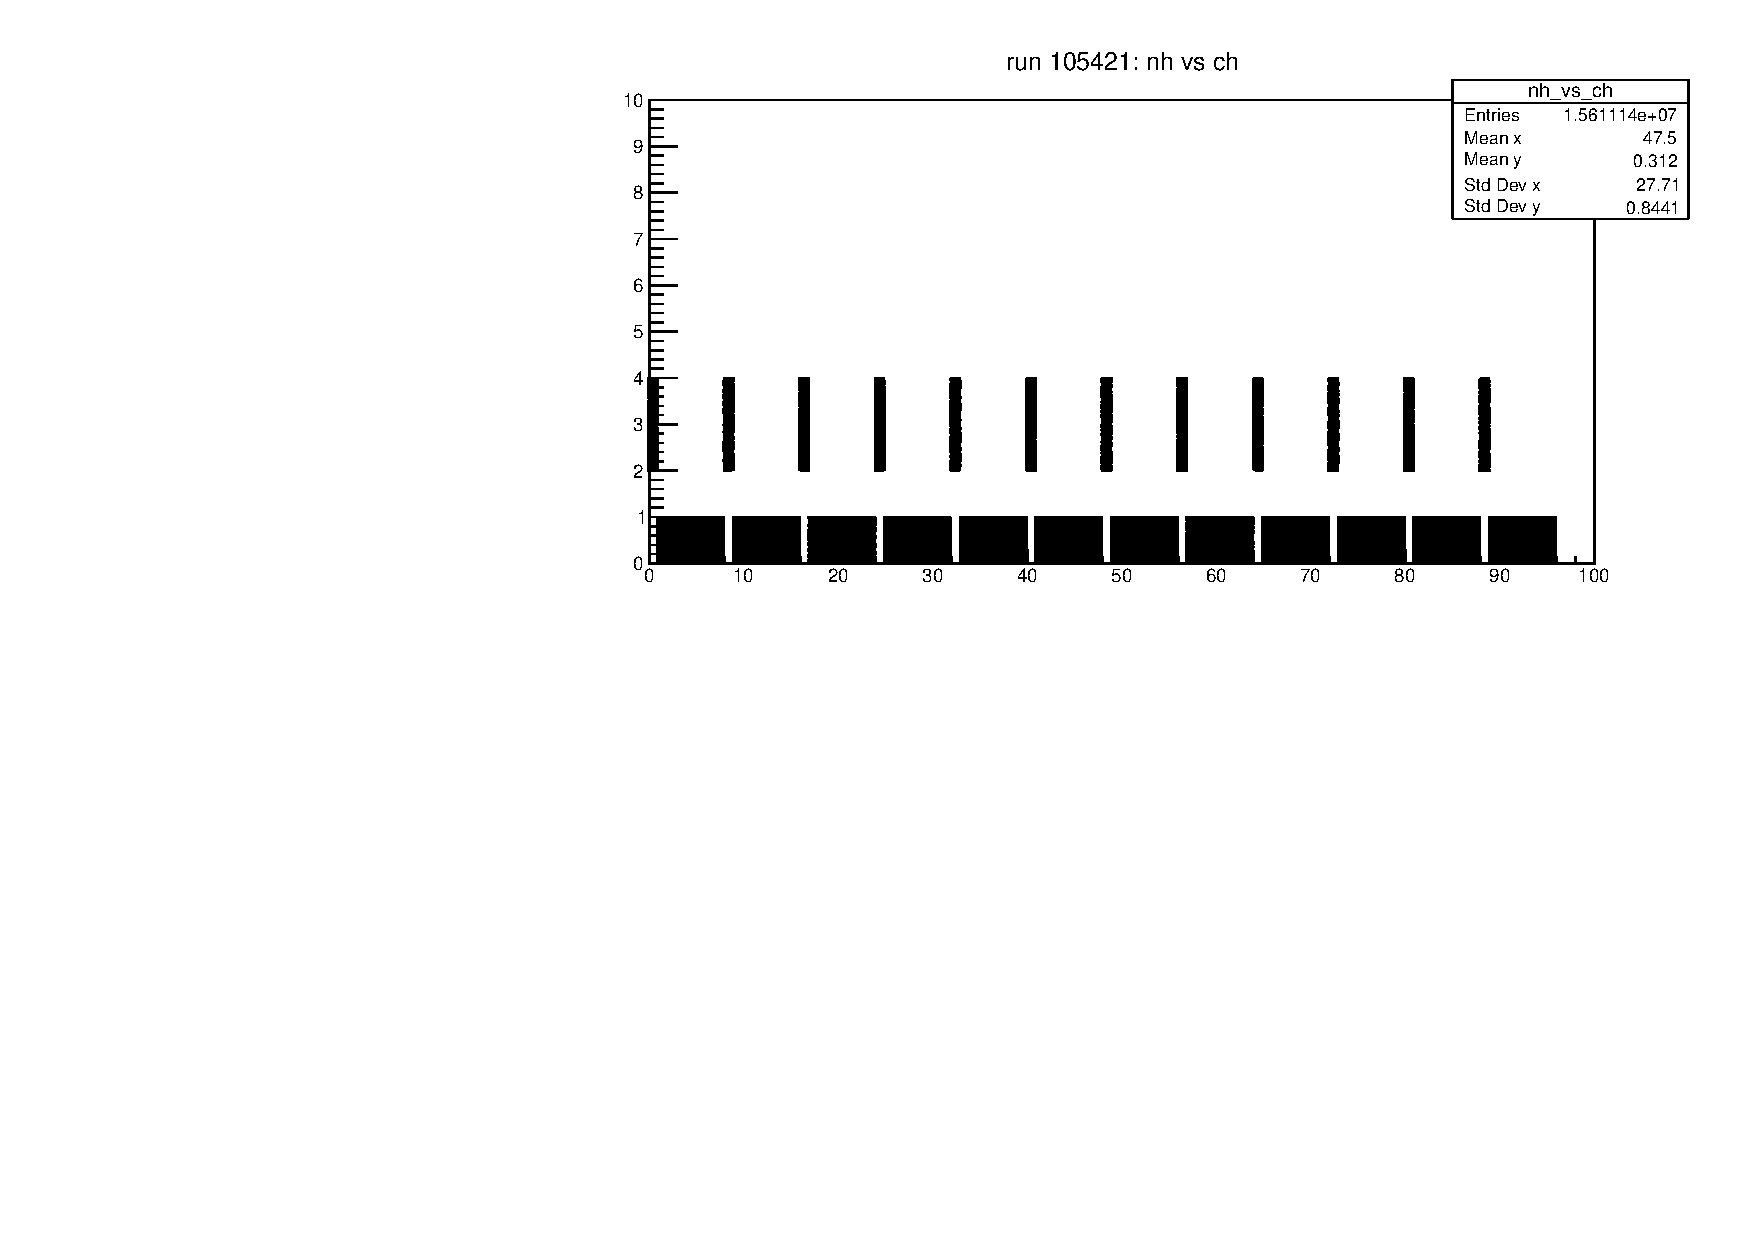
\includegraphics[width= 1.0\columnwidth]{figures/pdf/nhitsvsch_105421.pdf}
   \label{fig:wfgkghl}
 \end{figure}
\vspace{-6mm}
\begin{figure}[H]
   \centering
   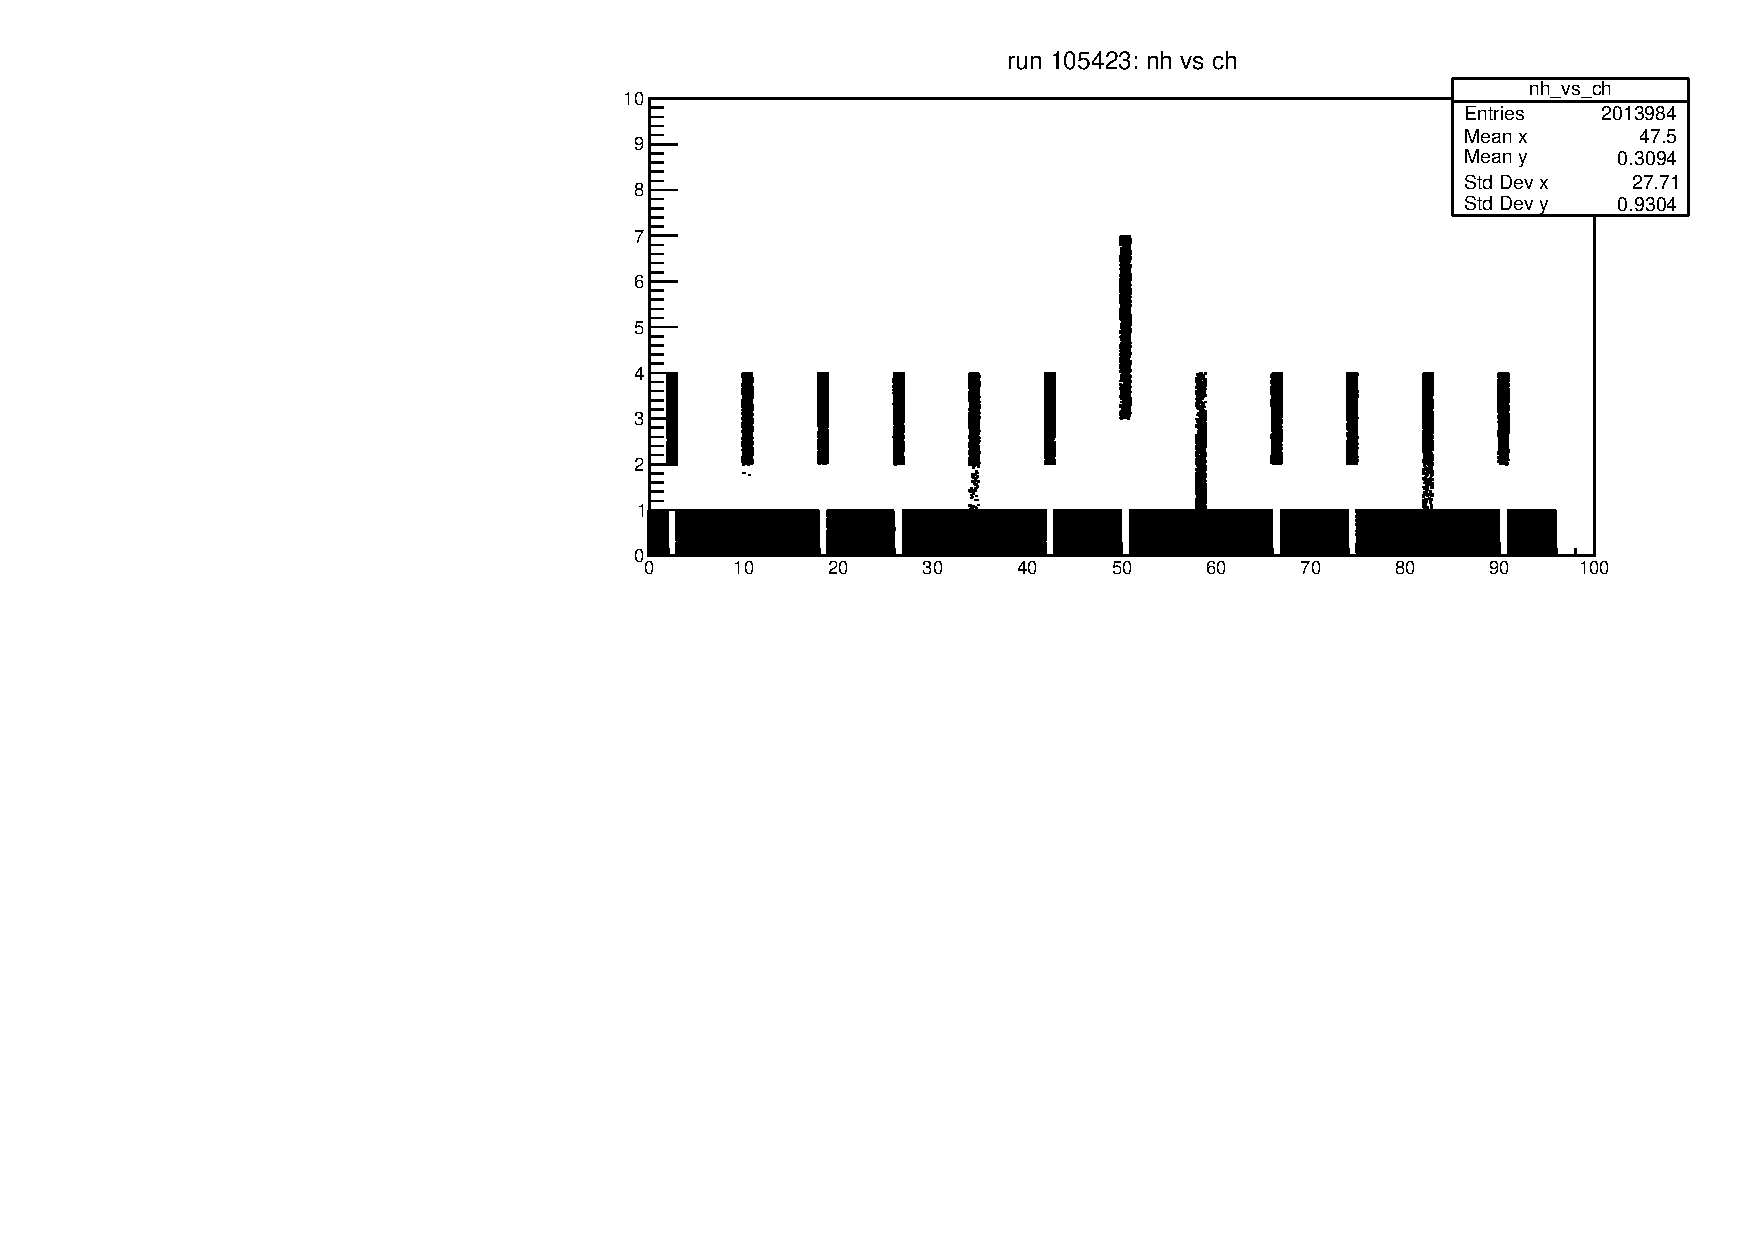
\includegraphics[width= 1.0\columnwidth]{figures/pdf/nhitsvsch_105423.pdf}
   \label{fig:wfgkgnvjkhl}
 \end{figure}
\end{column}
\begin{column}{0.5\framewidth}
\vspace{-7mm}
\begin{itemize}
\item  Cross talks in odd pulsed channels only;
\item  Asymmetric cross talks (e.g. 3$\rightarrow$5, not seen 3$\rightarrow$1).
\end{itemize}
\vspace{-4mm}
\begin{figure}[H]
   \centering
   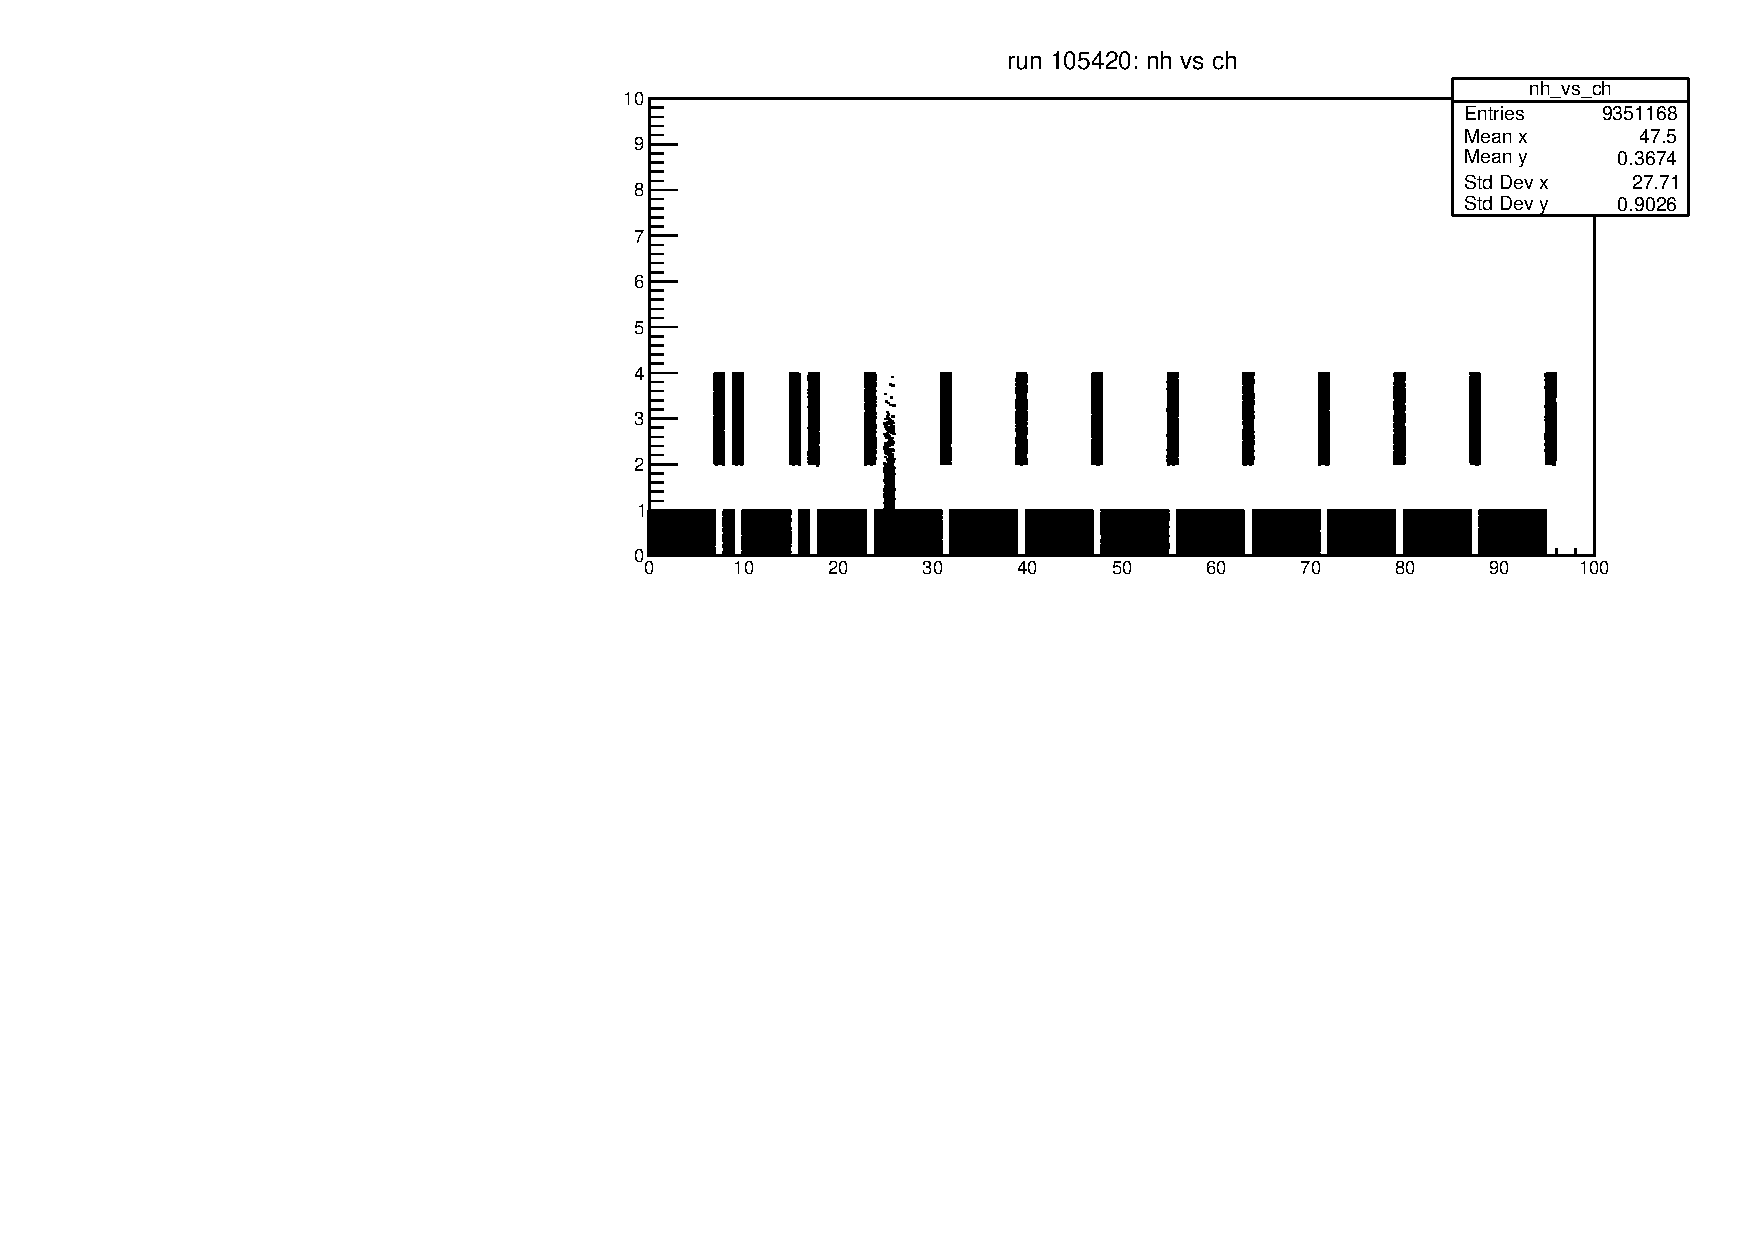
\includegraphics[width= 1.0\columnwidth]{figures/pdf/nhitsvsch_105420.pdf}
   \label{fig:wffytl}
 \end{figure}
\vspace{-4mm}
\begin{itemize}
\item DEAD channels found;
\item Less hits than expected;
\item More hits than expected:
\\
$\Rightarrow$ $\Delta t$ distribution;
\\
$\Rightarrow$ Negative waveforms.
\end{itemize}
\end{column}
\end{columns}

\end{frame}




\begin{frame}{Waveforms}
\vspace{-4mm}
\begin{columns}
\begin{column}{0.5\framewidth}
\begin{figure}[H]
   \centering
   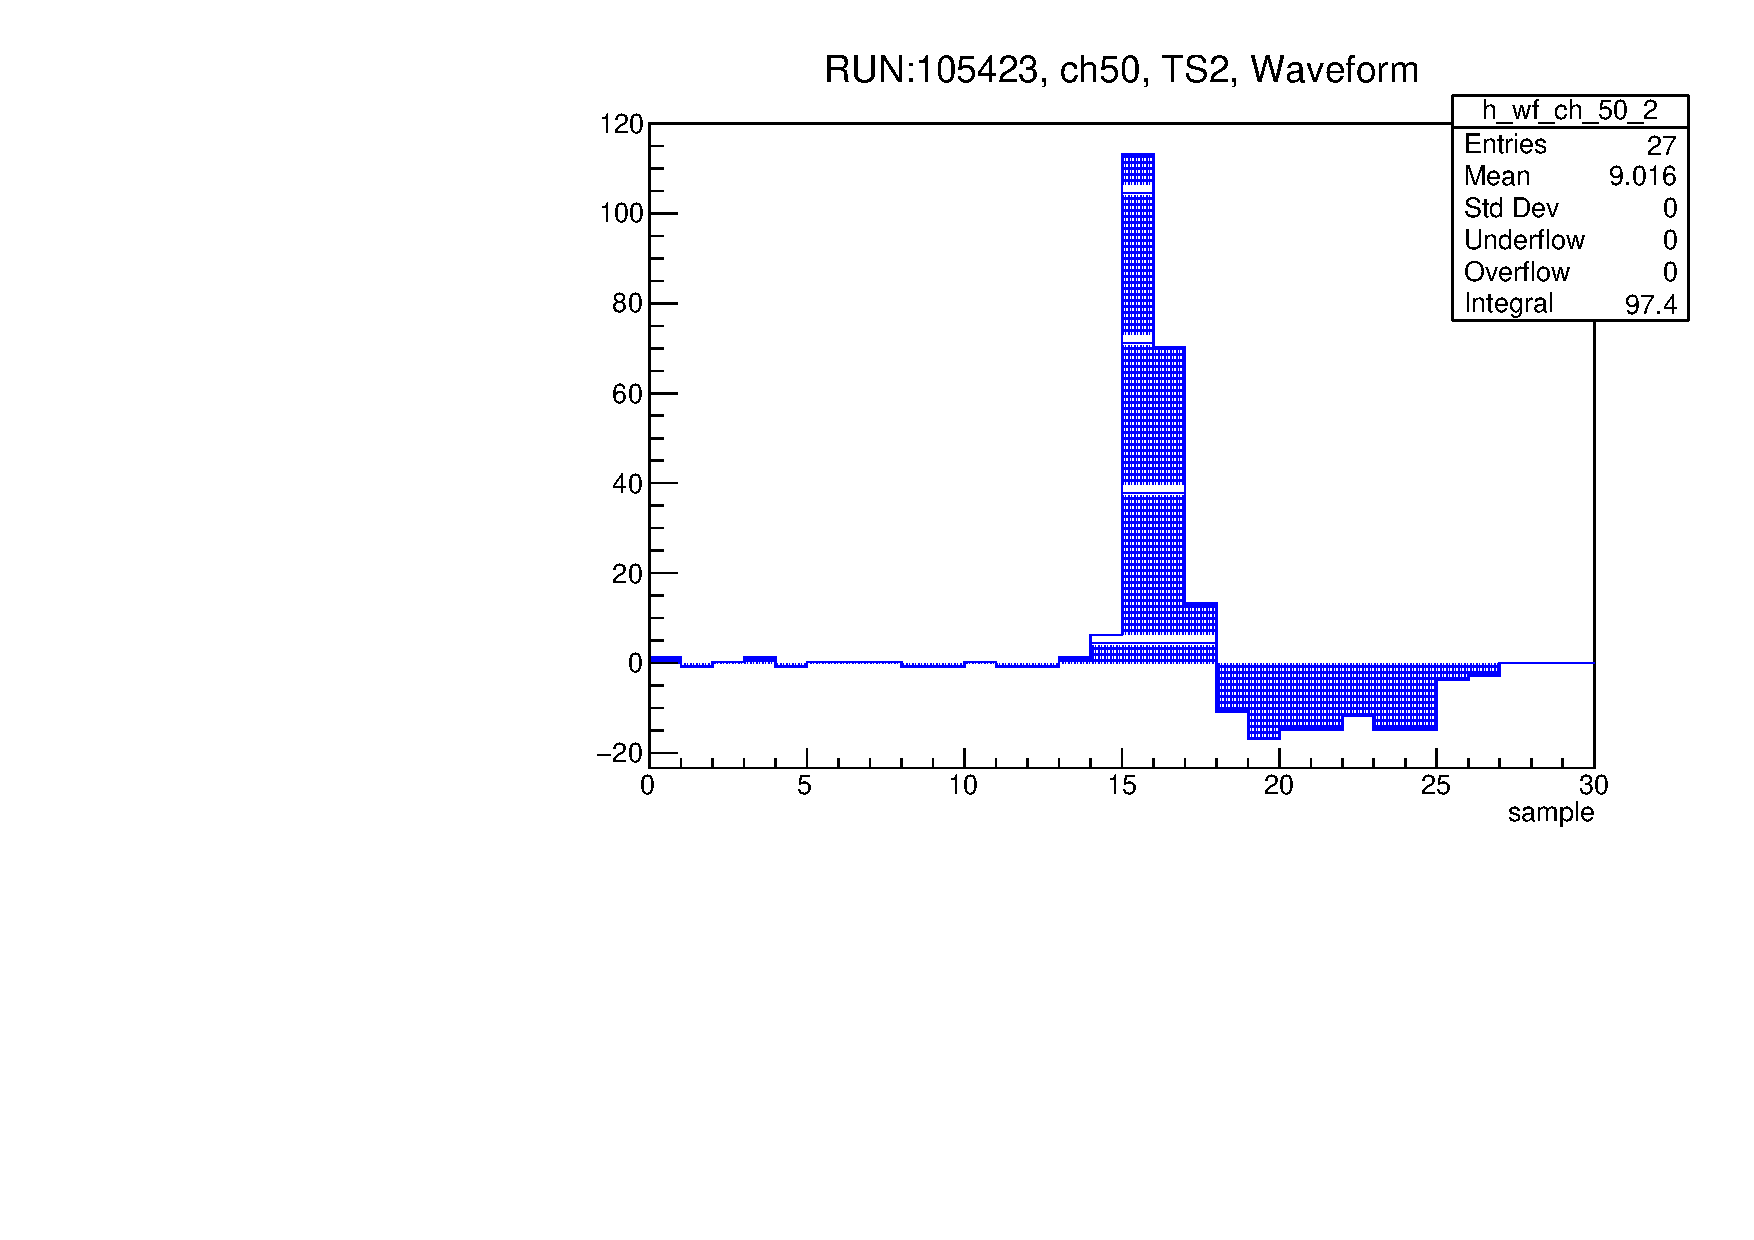
\includegraphics[width= 1.0\columnwidth]{figures/pdf/waveform_50_link_2.pdf}
   \label{fig:wfgkghl}
 \end{figure}
\vspace{-9mm}
\begin{figure}[H]
   \centering
   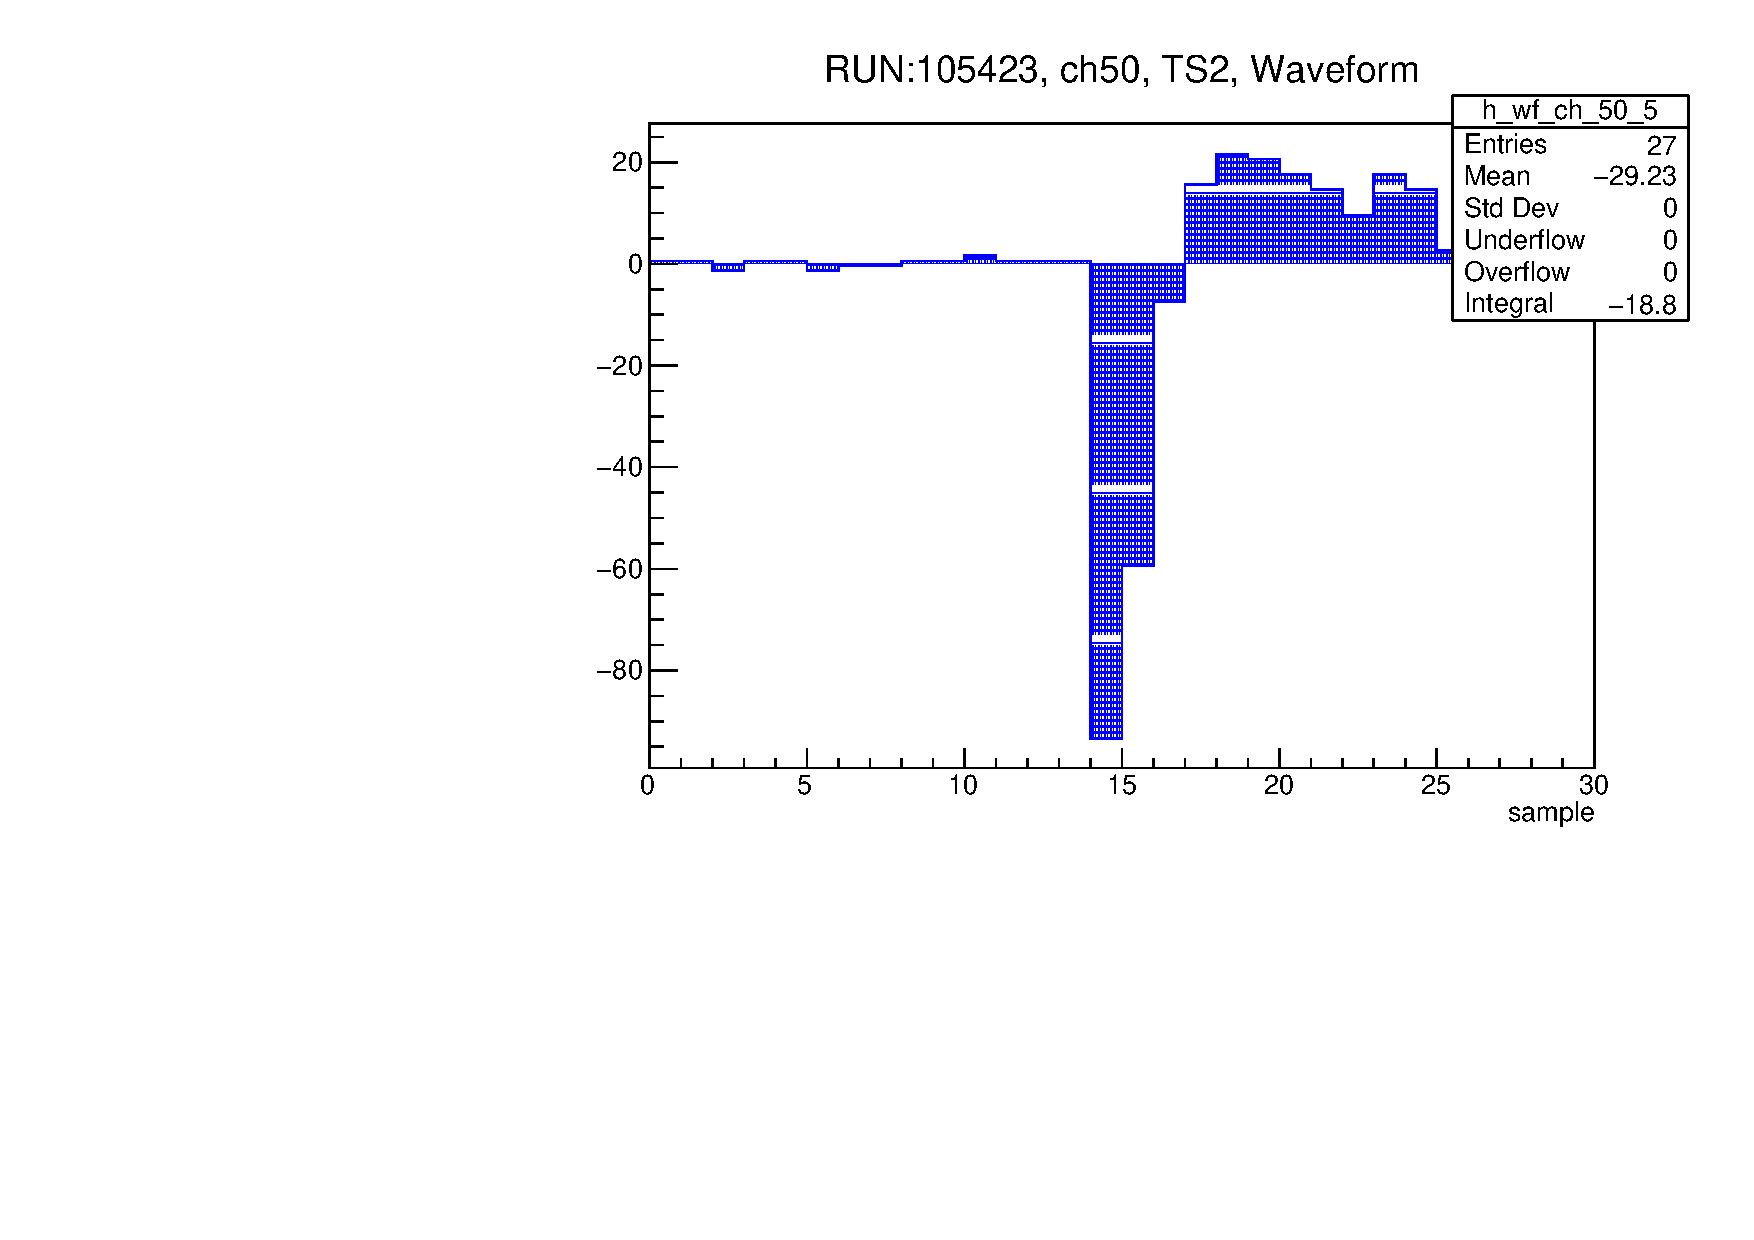
\includegraphics[width= 1.0\columnwidth]{figures/pdf/waveform_50_link_2_neg.pdf}
   \label{fig:wfgkgnvjkhl}
 \end{figure}
\end{column}
\begin{column}{0.5\framewidth}
\vspace{-7mm}
\begin{figure}[H]
   \centering
   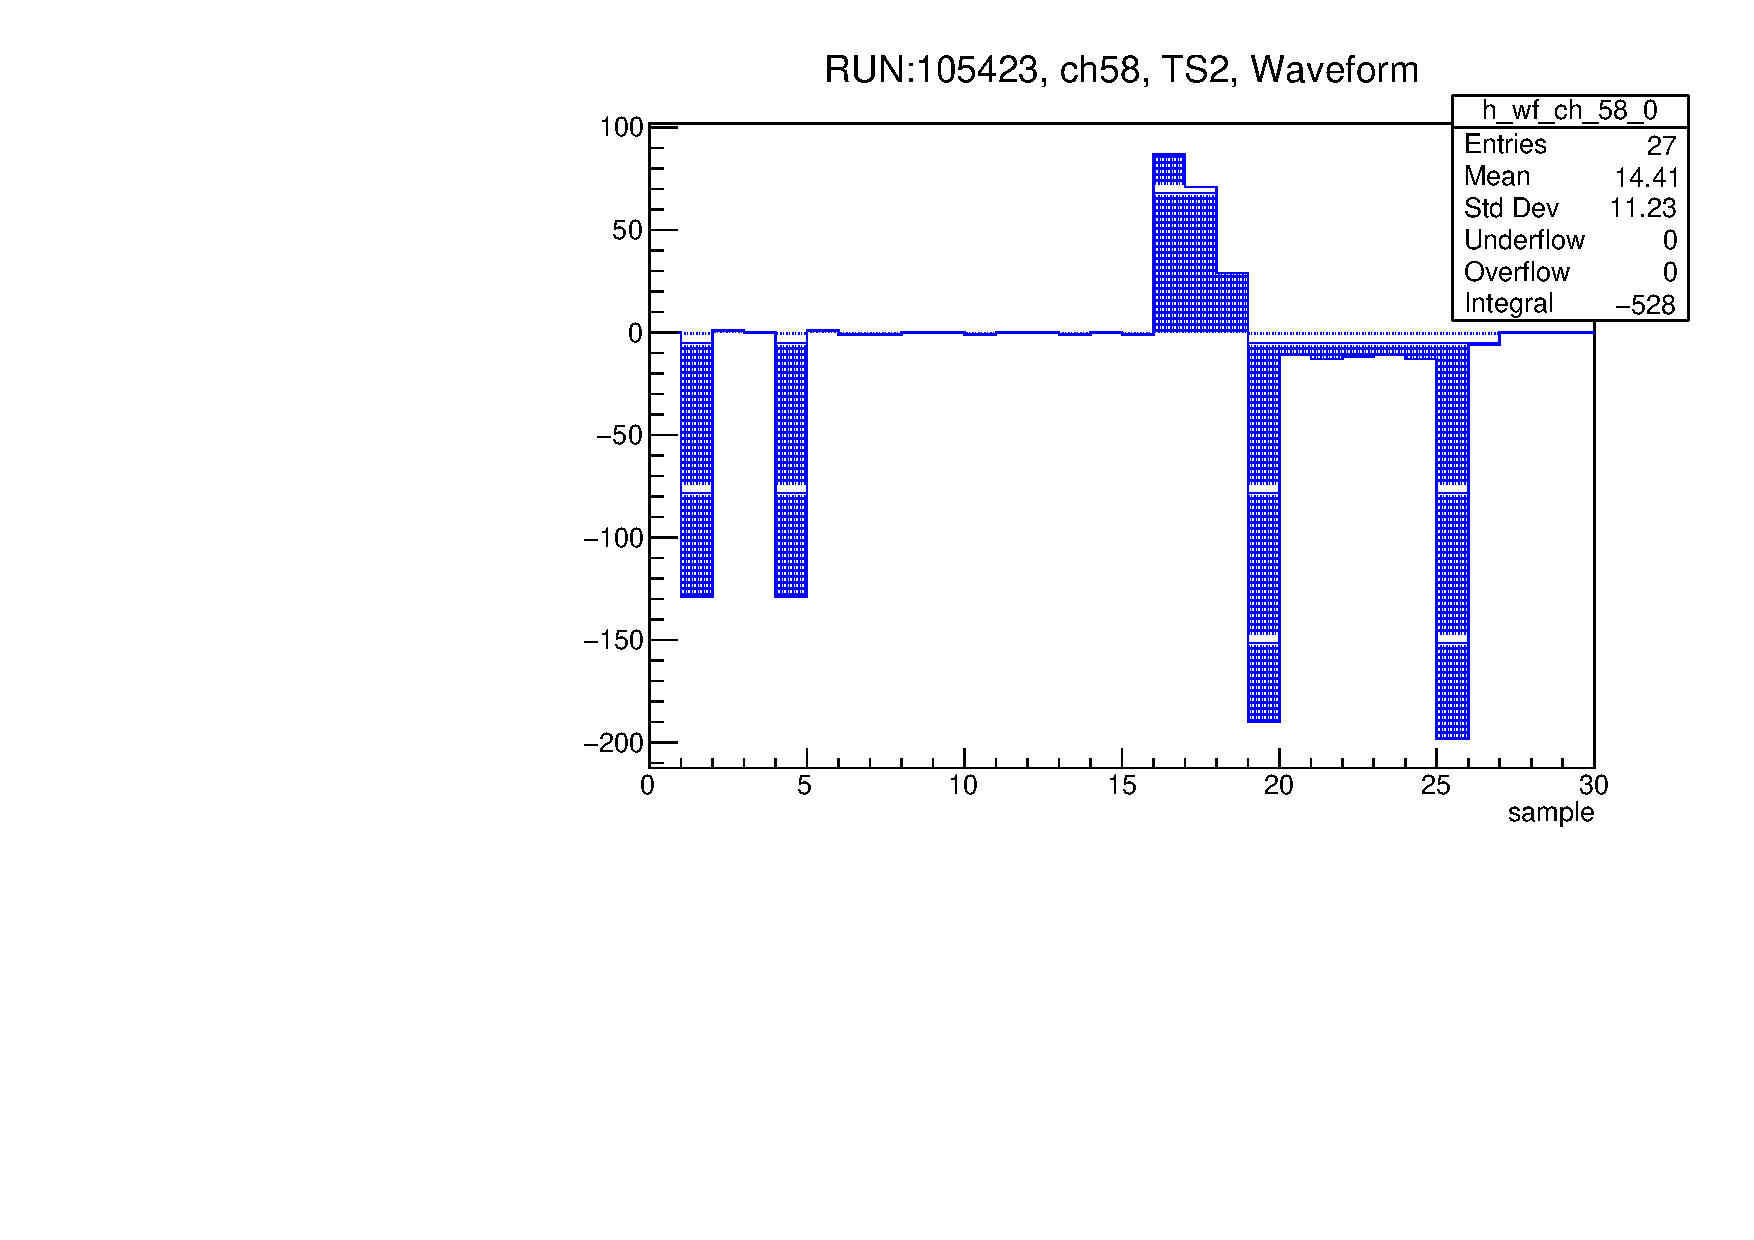
\includegraphics[width= 1.0\columnwidth]{figures/pdf/waveform_biterror.pdf}
   \label{fig:wffytl}
 \end{figure}
\begin{itemize}
{\tiny
\item Negative peaks (baseline and tail);
\item Peaks depth is 64, 128 or 192 (6th or/and 7th bit error);
\item Reconstruction of the waveforms: isolation of negative peaks;
\item The time interval between hits is always 20 $\mu$s for positive waveforms; 
\item Time difference distribution between hits for negative waveforms is peaked in 4 or 16 $\mu$s.}
\end{itemize}
\end{column}
\end{columns}
\end{frame}
\begin{frame}{Waveform Features versus Channel Number}
$q, \ ph, \ qt, \ fs$ mean value to identify critical channels (noisy channels, negative waveforms)
\begin{columns}
\begin{column}{0.5\framewidth}
\begin{figure}[H]
   \centering
   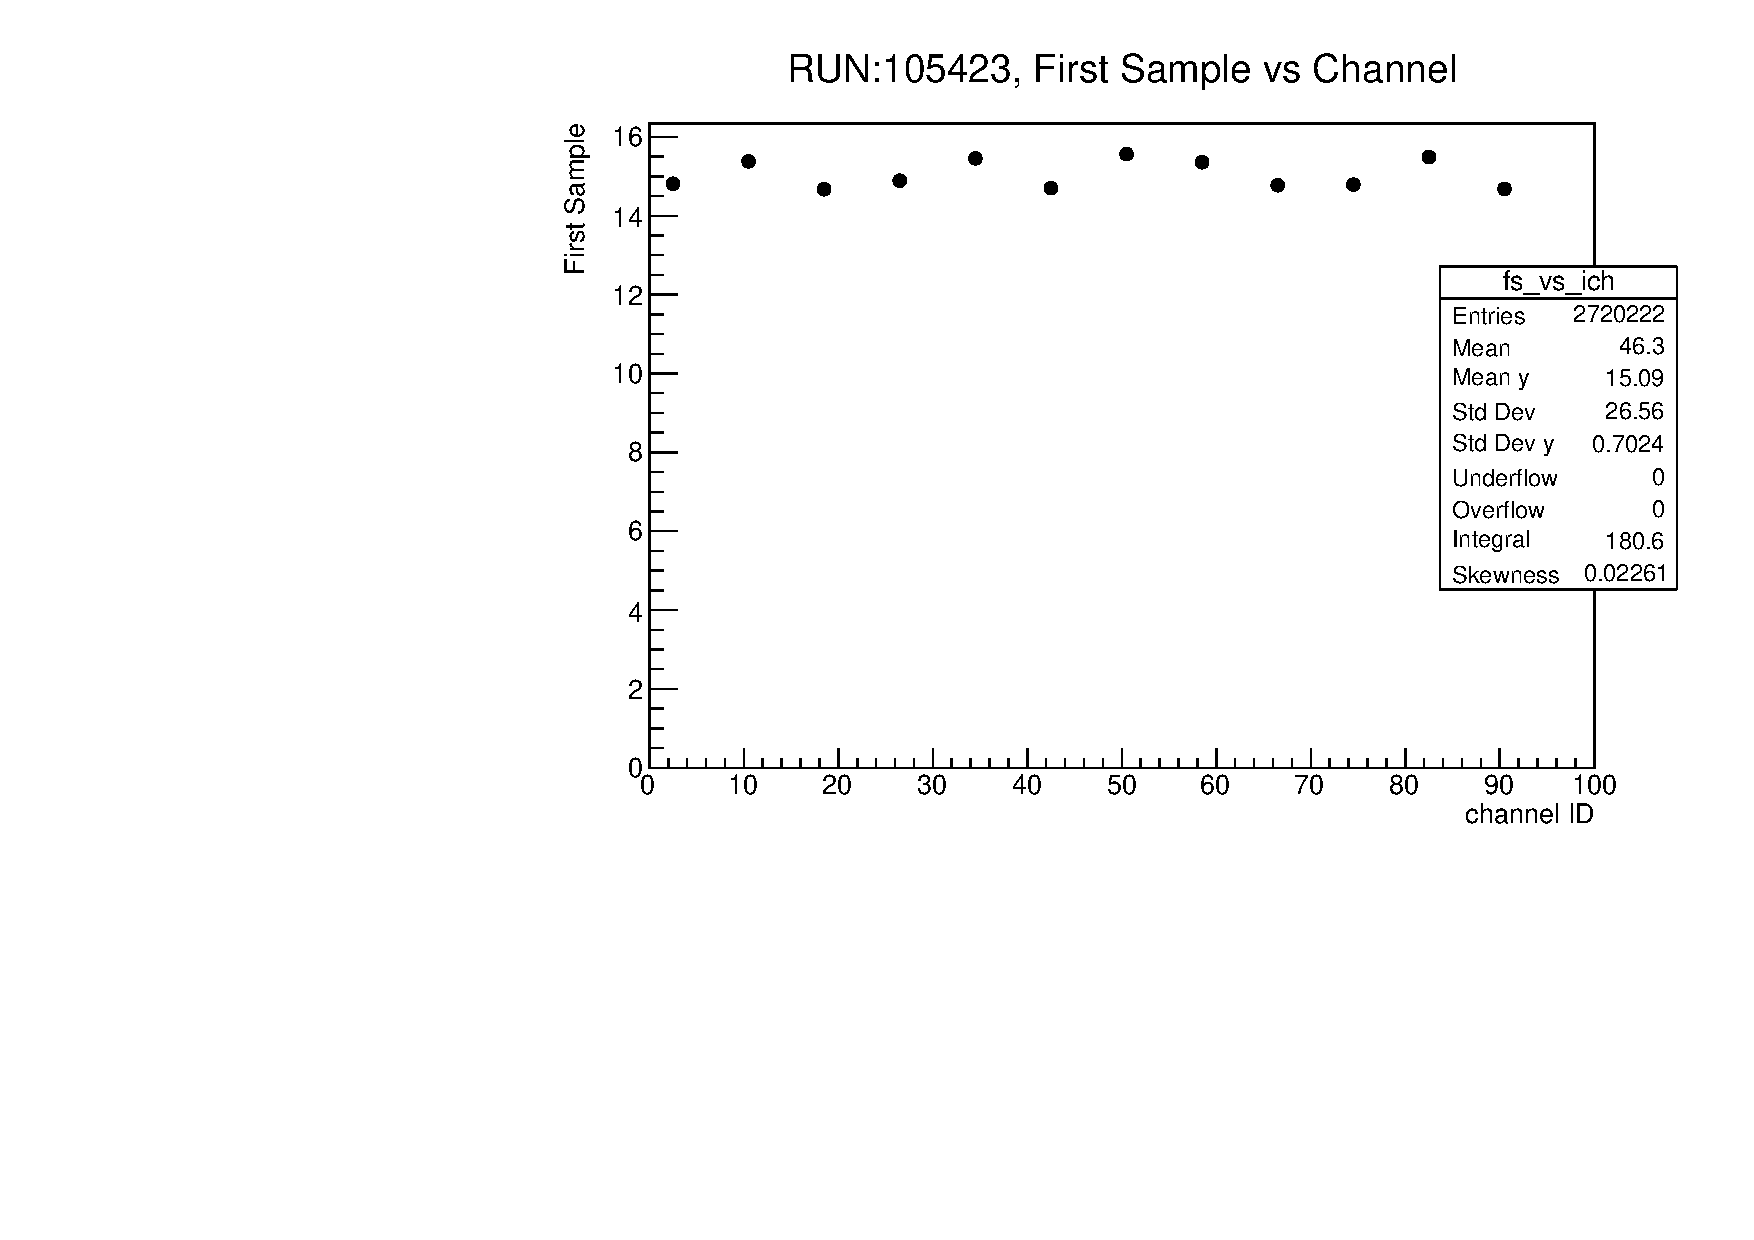
\includegraphics[width= 1.0\columnwidth]{figures/pdf/fs_vs_ch.pdf}
   \label{fig:wffytl}
 \end{figure}
\begin{figure}[H]
   \centering
   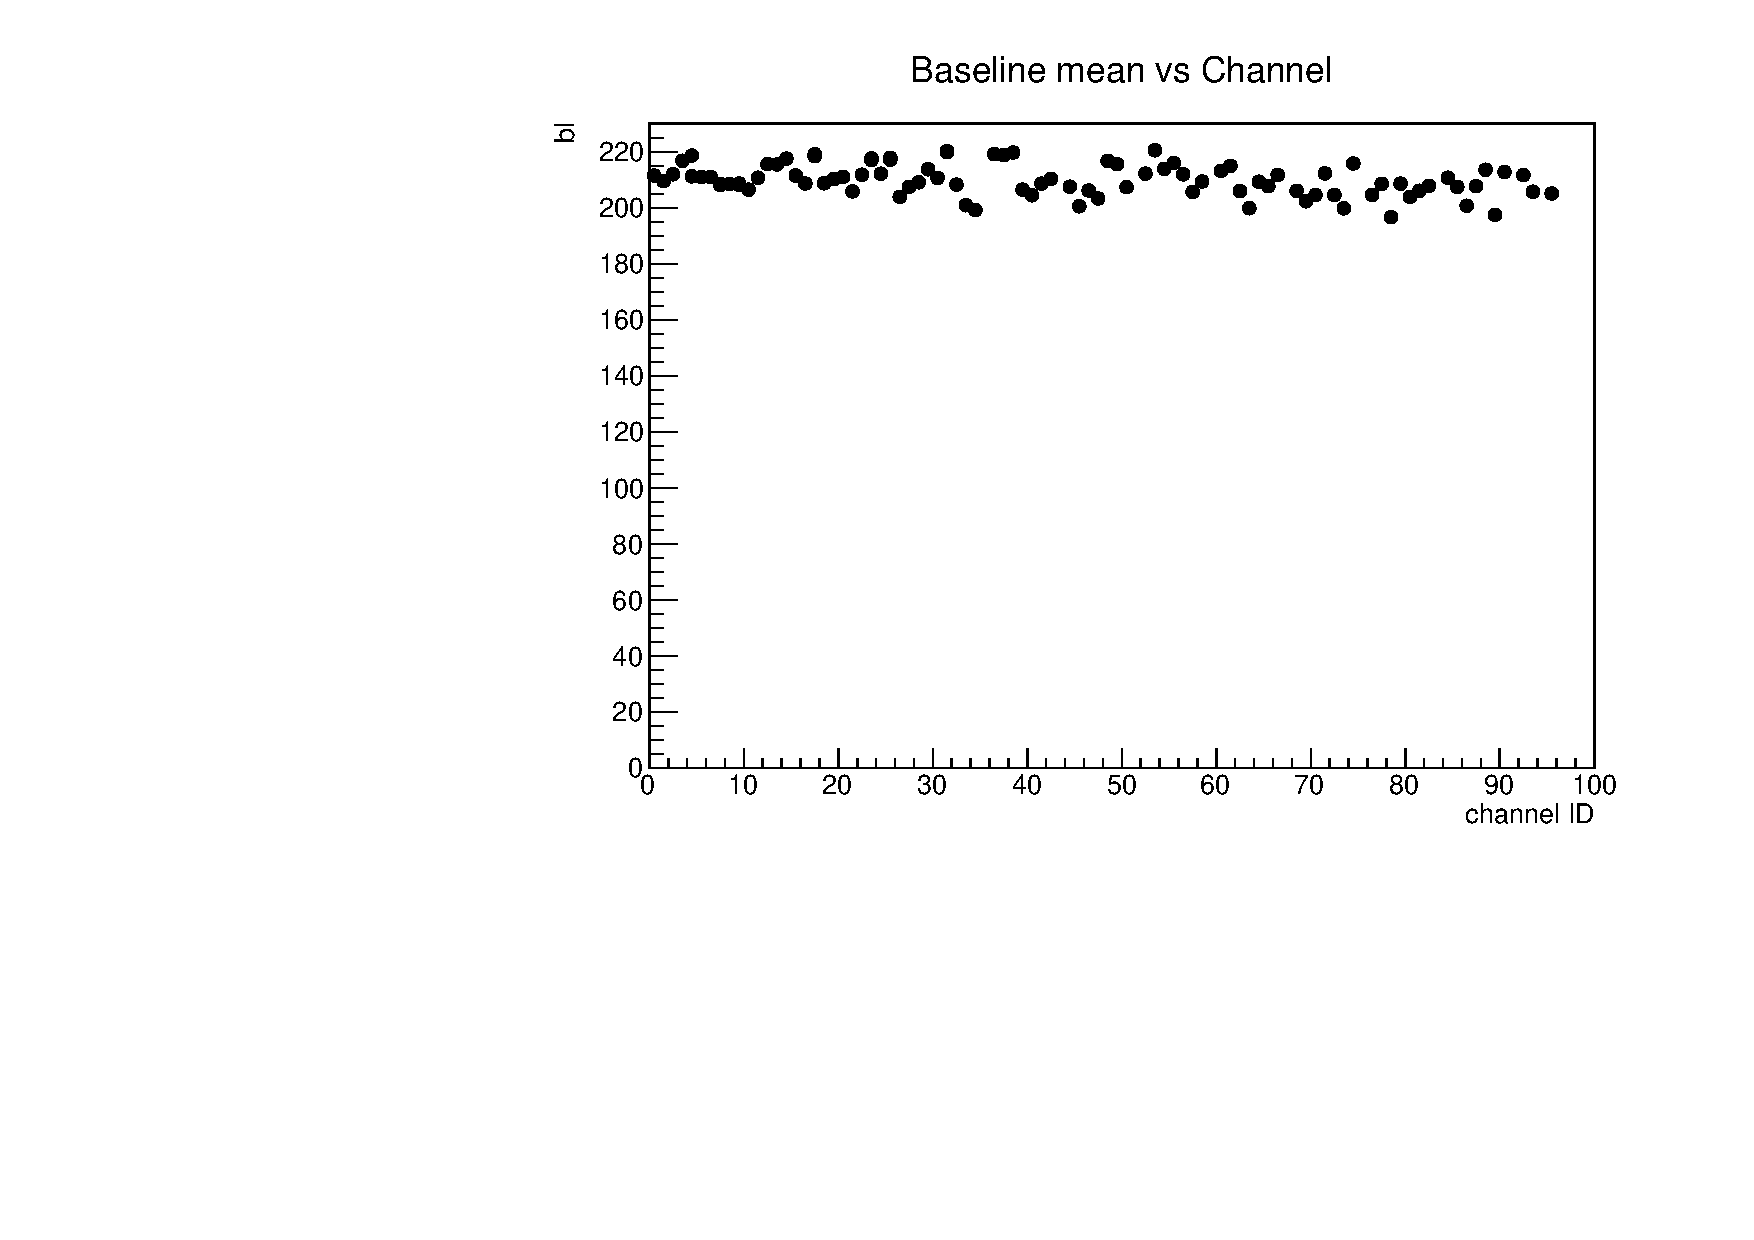
\includegraphics[width= 1.0\columnwidth]{figures/pdf/bl_vs_ch.pdf}
   \label{fig:wffytl}
 \end{figure}
\end{column}
\begin{column}{0.5\framewidth}
\begin{figure}[H]
   \centering
   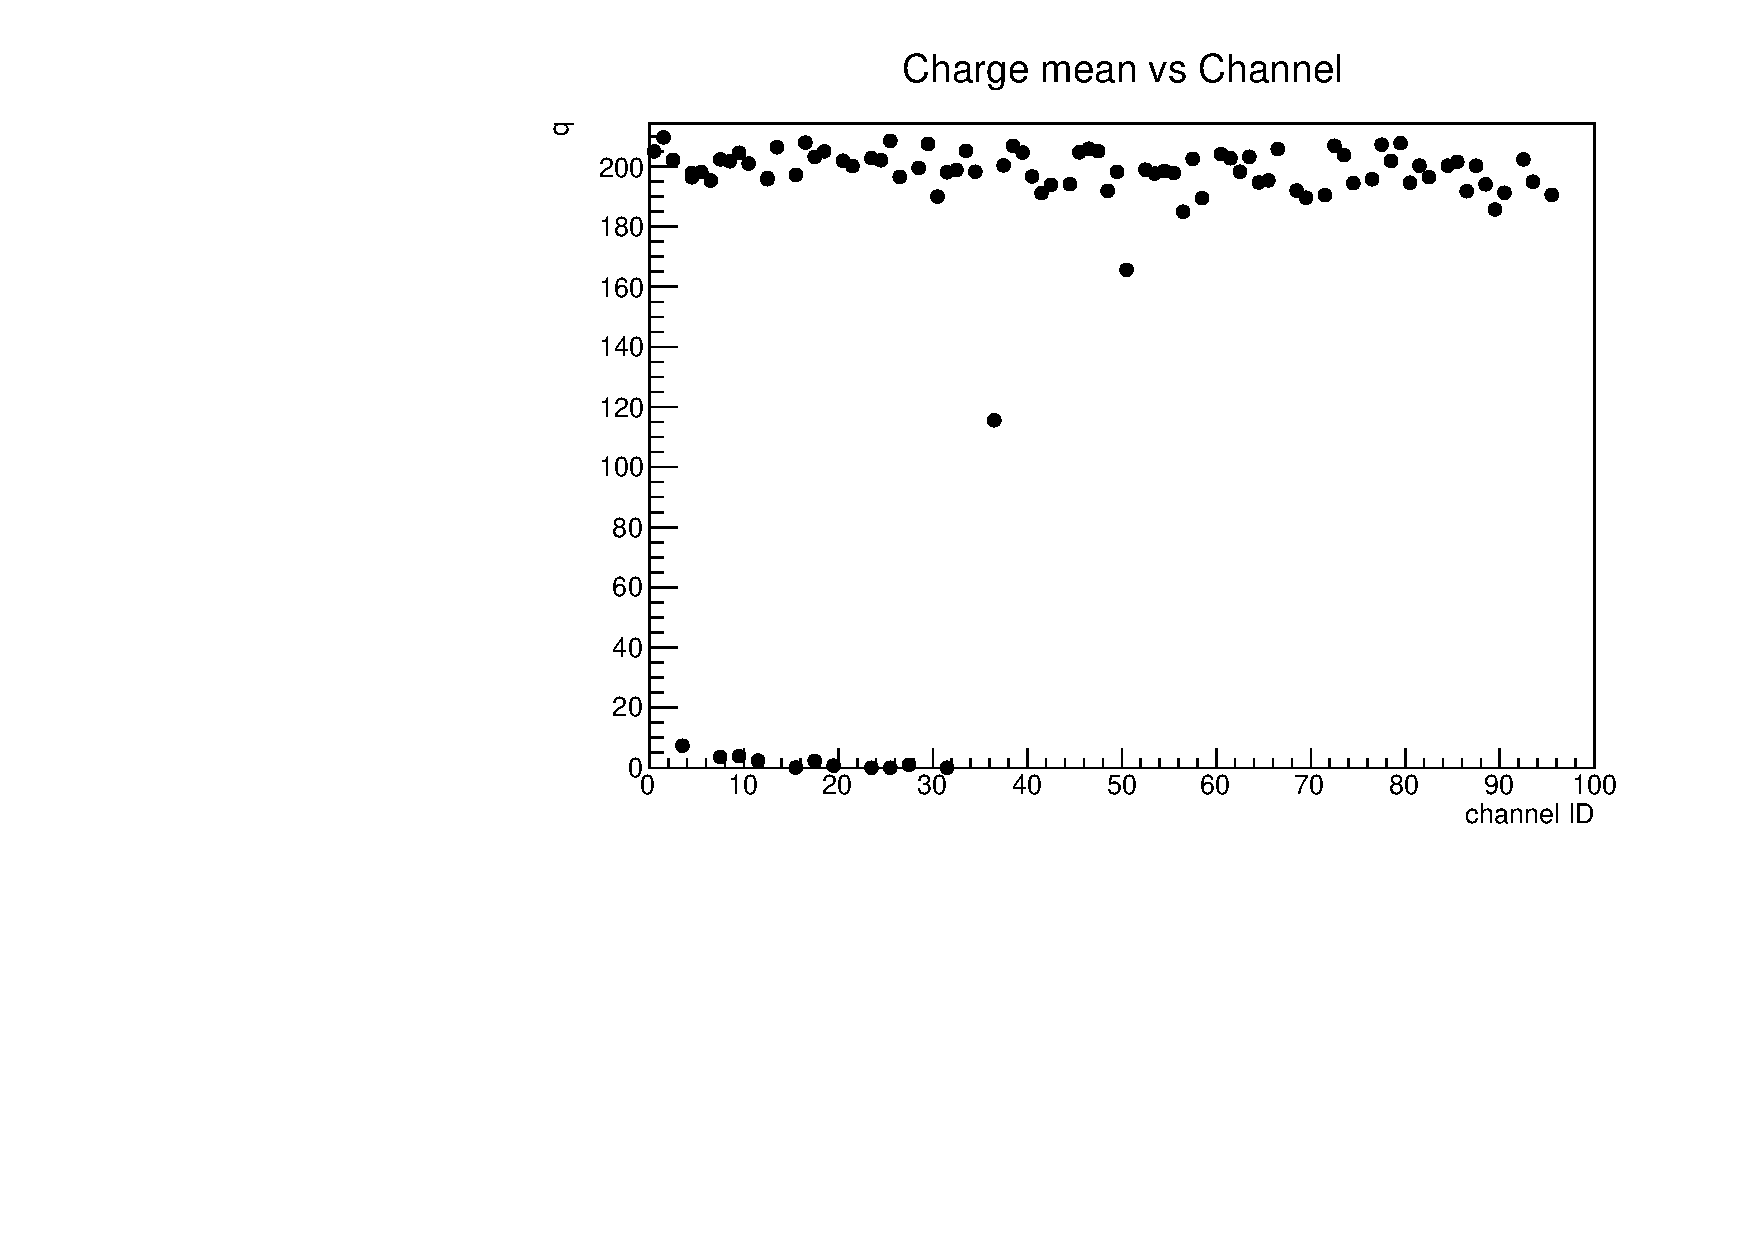
\includegraphics[width= 1.0\columnwidth]{figures/pdf/q_vs_ch.pdf}
   \label{fig:wffytl}
 \end{figure}
\begin{figure}[H]
   \centering
   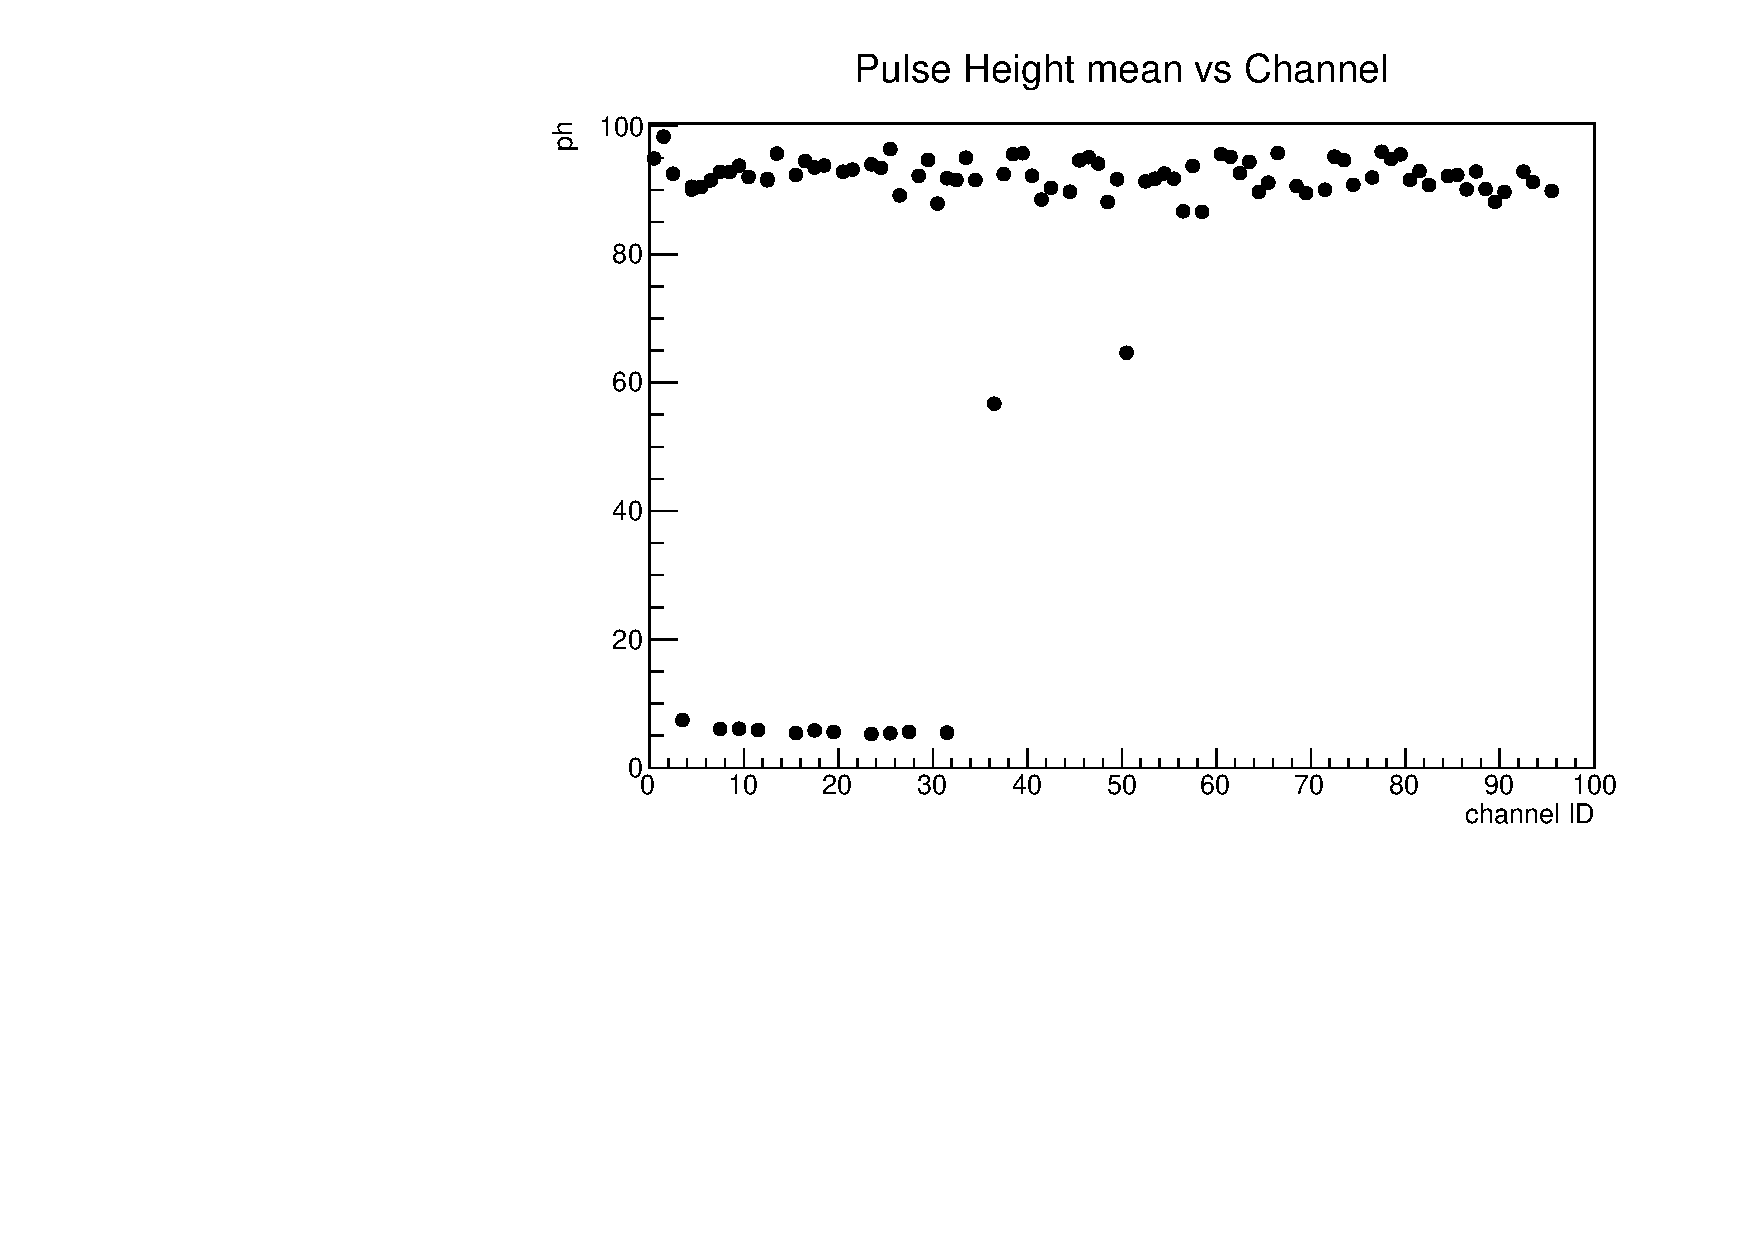
\includegraphics[width= 1.0\columnwidth]{figures/pdf/ph_vs_ch.pdf}
   \label{fig:wffytl}
 \end{figure}
\end{column}
\end{columns}
\end{frame}





\begin{frame}{Analysis of the charge and pulse height distribution}
\end{frame}

\iffalse
\begin{frame}{tmean}
\end{frame}
\begin{frame}{analysis of delta t between hits and negative waveforms}
lower value of charge and pulse height 
\end{frame}
\begin{frame}{more hits in one channel than 2/3}
\end{frame}
\begin{frame}{less hits in one channel than 2/3 and dead channels}
\end{frame}
\begin{frame}{glitches}
\end{frame}
\fi
\end{document}
